% ----------------------------------------------------------------------------
% B.2 --- Topological Configurations: Solitons as Particles
% From former B02, condensed
% ----------------------------------------------------------------------------
\subsection{Topological Configurations of the
\texorpdfstring{$\chi$}{χ} Field: Solitons as Particles}
\label{app:topological_solitons}

Solitonic configurations are effective geometric representations
illustrating how particle-like properties arise from stable, localized
configurations of $\chi_{\mathrm{eff}}$ once a smooth geometric
projection applies
(Appendix~\ref{app:relational_formulation}).

\subsubsection*{Charge as Oriented Relaxation Asymmetry}

A localized configuration deforms $\chi_{\mathrm{eff}}$ relative to
the background $\chi_{\mathrm{eff},0}$: excess (positive charge) or
deficit (negative charge).
The magnitude is diagnosed by a Gauss-like flux integral
$q_{\mathrm{eff}} \propto
  \oint_\Sigma \nabla\chi_{\mathrm{eff}} \cdot d\mathbf{S}$.
Coulomb-like interactions emerge from frustration minimization of the
Dirichlet functional
$\mathcal{F}[\chi_{\mathrm{eff}}]
  = \tfrac{1}{2}\int |\nabla\chi_{\mathrm{eff}}|^2\,d^3x$.

\begin{figure}[h]
  \centering
  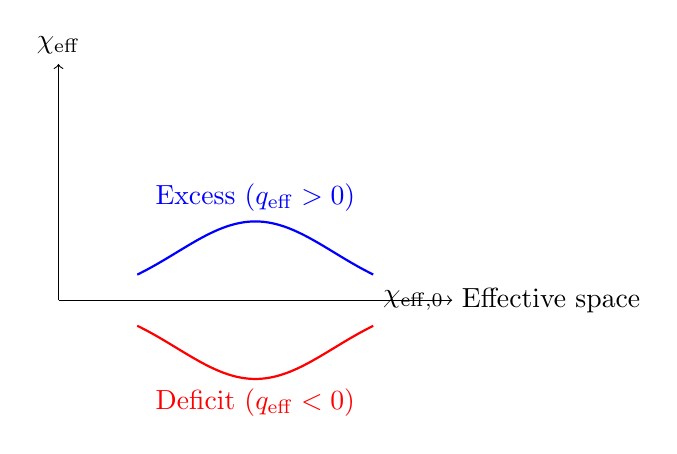
\begin{tikzpicture}[x=2cm, y=2cm]
    \draw[->] (0,0) -- (2.5,0)
      node[right] {Effective space};
    \draw[->] (0,0) -- (0,1.5)
      node[above] {$\chi_{\mathrm{eff}}$};
    \draw[thick, blue, domain=0.5:2, samples=100]
      plot (\x, {0.5*exp(-2*(\x-1.25)^2)});
    \node[blue, above] at (1.25, 0.5)
      {Excess ($q_{\mathrm{eff}}>0$)};
    \draw[thick, red, domain=0.5:2, samples=100]
      plot (\x, {-0.5*exp(-2*(\x-1.25)^2)});
    \node[red, below] at (1.25, -0.5)
      {Deficit ($q_{\mathrm{eff}}<0$)};
    \draw[dashed] (0.5,0) -- (2,0);
    \node[right] at (2,0)
      {$\chi_{\mathrm{eff},0}$};
  \end{tikzpicture}
  \caption{Oriented deformations of
    $\chi_{\mathrm{eff}}$ defining effective charge
    polarity.}
  \label{fig:chi_charges}
\end{figure}

\subsubsection*{Vortical Configurations and Integer-Spin
Excitations}
\label{subsec:vortices}

An effective winding number
$n = (2\pi)^{-1}
  \oint \nabla\arg(\chi_{\mathrm{eff}}) \cdot d\mathbf{l}$
characterizes charge orientation, topological robustness, and integer
spin.

\begin{figure}[h]
  \centering
  \begin{tikzpicture}[x=2cm, y=2cm]
    \draw[->] (-1.5,0) -- (1.5,0) node[right] {$x$};
    \draw[->] (0,-1.5) -- (0,1.5) node[above] {$y$};
    \foreach \r in {0.2,0.4,...,1.2} {
      \draw[blue, thick, domain=0:6.28, samples=100]
        plot ({\r*cos(\x)}, {\r*sin(\x)});
    }
    \fill[red] (0,0) circle (0.05);
    \node[red, below] at (0,0) {Core};
    \node[blue] at (1.2,1.2) {$n=1$};
  \end{tikzpicture}
  \caption{Vortical configuration with winding $n=1$
    (integer spin).}
  \label{fig:chi_vortex}
\end{figure}

\subsubsection*{Skyrmion-Like Configurations and
Spin-$\tfrac{1}{2}$ Excitations}
\label{subsec:skyrmions}

Configurations with topological index $Q = \pm 1$ exhibit
$4\pi$-periodicity under rotations, providing a geometric origin for
spin-$\tfrac{1}{2}$ behavior and fermionic statistics.

\begin{figure}[h]
  \centering
  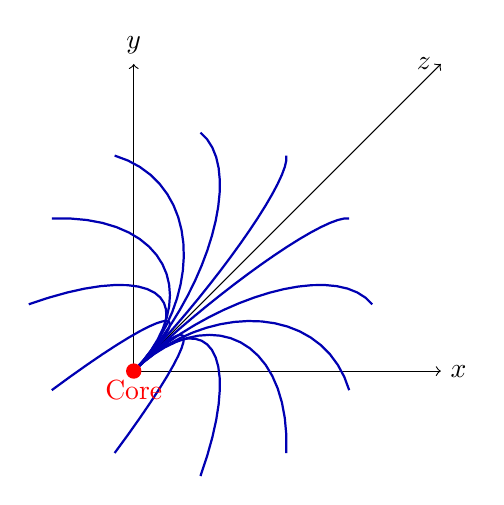
\begin{tikzpicture}[x=1.5cm, y=1.5cm, z=1.5cm,
    scale=1.3]
    \draw[->] (0,0,0) -- (2,0,0) node[right] {$x$};
    \draw[->] (0,0,0) -- (0,2,0) node[above] {$y$};
    \draw[->] (0,0,0) -- (0,0,2) node[left] {$z$};
    \foreach \phi in {0,30,...,330} {
      \draw[blue!70!black, thick,
        domain=0:1.2, samples=20]
        plot ({
          \x*sin(\x r)*cos(\phi)},
          {\x*sin(\x r)*sin(\phi)},
          {\x*cos(\x r)});
    }
    \fill[red] (0,0,0) circle (0.05);
    \node[red, below] at (0,0,0) {Core};
  \end{tikzpicture}
  \caption{Skyrmion-like configuration of
    $\chi_{\mathrm{eff}}$ (spin-$\tfrac{1}{2}$).}
  \label{fig:chi_skyrmion}
\end{figure}

\subsubsection*{Summary: Topology, Charge, and Spin}

\begin{table}[htbp]
  \centering
  \caption{Effective solitonic configurations and
    emergent particle properties.}
  \label{tab:solitons_charge}
  \begin{tabular}{|c|c|c|c|}
    \hline
    \textbf{Configuration} &
    \textbf{Index} &
    \textbf{$\chi_{\mathrm{eff}}$ asymmetry} &
    \textbf{Properties} \\
    \hline
    Vortical & $n$ &
    Excess/deficit &
    Charge $\propto n$, int.\ spin \\
    \hline
    Skyrmion & $Q=\pm 1$ &
    Oriented deformation &
    Charge $\propto Q$, spin-$\tfrac{1}{2}$ \\
    \hline
  \end{tabular}
\end{table}
